\documentclass[preprint,12pt,3p]{elsarticle}
\usepackage{epsfig,amssymb,amsfonts,amsmath,mathtools,bm}
\biboptions{sort&compress}

\newcommand{\X}{X(3872)}
\newcommand{\vep}{{\bm p}}
\newcommand{\vek}{{\bm k}}
\newcommand{\veq}{{\bm q}}
\newcommand{\ves}{{\bm s}}
\newcommand{\veg}{{\bm g}}
\newcommand{\veY}{{\bm Y}}
\newcommand{\ven}{{\bm n}}
\newcommand{\ver}{{\bm r}}
\newcommand{\vej}{{\bm j}}
\newcommand{\vel}{{\bm l}}
\newcommand{\veS}{{\bm S}}
\newcommand{\veA}{{\bm A}}
\newcommand{\veep}{{\bm \epsilon}}
\newcommand{\h}{\vphantom{$\int_0^1$}}
\newcommand{\be}{\begin{equation}}
\newcommand{\ee}{\end{equation}}
\newcommand{\bea}{\begin{eqnarray}}
\newcommand{\eea}{\end{eqnarray}}
\newcommand{\beas}{\begin{eqnarray*}}
\newcommand{\eeas}{\end{eqnarray*}}
\newcommand{\Br}{{\rm Br}}
% \newcommand{\dis}{\displaystyle}
\newcommand{\ds}{\displaystyle}
\newcommand{\0}{}
%\newcommand{\0}{^{\rm{ph}}}
% \newcommand{\oo}[1]{(#1^{\rm ph})^2}
\usepackage[active]{srcltx}

\DeclareMathSymbol{\varGamma}{\mathord}{letters}{"00}
\journal{Physics Letters B}
\begin{document}

While very successful in many aspects, the Standard Model of particle physics (SM)
leaves a couple of important questions unanswered. On the one hand, it predicts
an amount of matter that survived annihilation after the Big Bang that is many orders
of magnitude less compared to what is observed. In addition, since masses
of matter particles appear as parameters in the SM, it does not provide any understanding
why the values of these masses span so many orders of magnitude.
In addition, within the SM phenomena like Dark Matter and Dark Energy can not be explained.
 These and some more 
issues suggest that there must be physics beyond the SM, and many experiments
world-wide hunt for signals of it. 

One of the currently most promising candidates to provide a signal for physics beyond the SM
is the muon anomaly $a_\mu = (g-2)/2$. It is a low-energy observable, which
can be both measured and computed to high precision~\cite{Jegerlehner:2009ry,Blum:2013xva}.  The present experimental
value $a_\mu^{EXP}= 1\ 165\ 920\ 89 (63)\times 10^{-11}$
 comes from the BNL E821 experiment~\cite{Bennett:2006fi}.  This value
deviates from the SM prediction by about 3 standard
deviations $\Delta a_\mu^{({\rm EXP-SM})}= (287\pm 80)\times 10^{-11}$~\cite{Davier:2010nc} 
or $= (261\pm 78)\times 10^{-11}$~\cite{Hagiwara:2011af}, depending on how the leading-order
hadronic contributions are evaluated.  While this discrepancy
is not large enough to claim a failure of the SM, it is currently the largest
deviation of a SM prediction from an experimental observable. This
alone justifies all efforts currently taken to improve both the theoretical as well as the experimental value.
New measurements are planned within the next four years at 
Fermilab/USA~\cite{Grange:2015fou} and also at JPARC/Japan~\cite{Saito:2012zz}. The goal
of the measurements is to reduce the uncertainty by a factor of four. 
In parallel the SM prediction needs to be improved in accuracy 
 by at least a factor of two to establish a deviation from the SM for the first time.
 

The largest uncertainty of the SM prediction comes from
 the hadronic quantum corrections~\cite{Jegerlehner:2009ry}.
At the level of accuracy that is relevant at the moment the hadronic
contributions can be split up into the hadronic vacuum polarization
(HVP), displayed on the left-hand side of figure \ref{fig:gm2}, and the
hadronic light-by-light scattering (HLbL), displayed in the middle of
Fig.~\ref{fig:gm2}. The most important contribution to the latter
comes from the pseudoscalar pole contributions, displayed explicitly on the right-hand 
side of Fig.~\ref{fig:gm2}. For those one expects that the contribution
should be largely saturated by the lightest exchange particles, namely the 
$\pi^0$, the $\eta$ and the $\eta'$. 
%
\begin{figure}[!h]
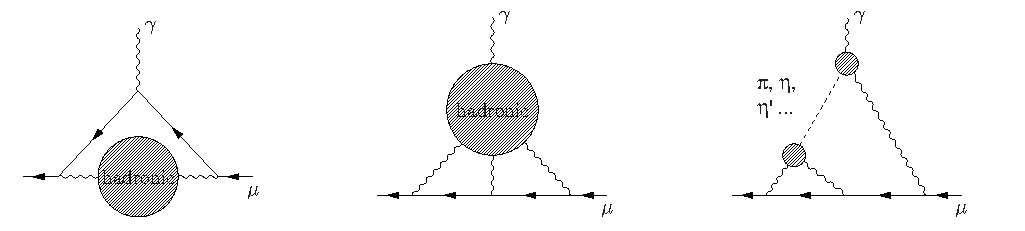
\includegraphics[keepaspectratio,width=1.\textwidth]{figures/intro/hadronicgm2.pdf}
\caption{Hadronic contributions to $a_\mu$: hadronic vacuum polarization (left diagram), 
  hadronic light-by-light scattering (middle), pion-pole contribution to hadronic light-by-light scattering (right). 
  Full lines with an arrow denote muons, wiggly lines photons, the dashed line a pseudo-scalar meson and shaded blobs a non-pointlike 
  hadronic substructure.
}
\label{fig:gm2}
\end{figure}

Concerning the SM prediction for $a_\mu$ HLbL is suppressed relative to HVP by one power of the electromagnetic
fine structure constant~\cite{Jegerlehner:2009ry,Bijnens:2007pz}.  
Unfortunately at present it is not possible to straightforwardly 
calculate the contributions shown in Fig.~\ref{fig:gm2} 
from first principles analogously to, e.g., the QED corrections, since
  both processes concern low-energy corrections,
i.e.\ non-perturbative physics. Thus the prime candidate for a SM
calculation of hadronic corrections seems to be lattice QCD~\cite{Gattringer:2010zz}. 
However, it is not expected that lattice QCD
results for HPV will reach the required accuracy in the foreseeable future.
For the HLbL only preliminary lattice-QCD calculations have been reported~\cite{Blum:2014oka}.  
In view of the challenges to determine
a four-point function that includes in addition disconnected diagrams
it is not clear yet when a profound lattice calculation with
controlled uncertainties and a reliable error estimate will be
available.

Fortunately there is an alternative way to quantify hadronic corrections. It requires both
theoretical as well as experimental efforts:
Dispersion theory provides a link between particular hadronic cross sections
and $a_\mu$---for a discussion of the HVP in this context see Ref.~\cite{Jegerlehner:2009ry}, while 
for HLbL we refer to Refs.~\cite{Colangelo:2014dfa,Pauk:2014rfa,Colangelo:2014pva,Colangelo:2015ama}.  
In particular for the latter contribution it allows one to calculate from the transition
form factors of the kind $\pi^0$, $\eta$, $\eta'\to \gamma^*\gamma^*$ 
the corresponding piece for the meson pole contribution as displayed in the
right most diagram of Fig.~\ref{fig:gm2}.
The measurements proposed here provide important information towards
the necessary input needed for the evaluation of the HLbL contribution, since
$\eta'\to \gamma^*\gamma$ gives the single off-shell form factor of the $\eta'$
and $\phi\to \eta\gamma$ additionally provides information on the isoscalar
piece of $\eta\to \gamma^*\gamma$ in a different kinematic regime.
Additional information on the  $\eta$ and
$\eta'$ form factors can be found from the dispersive methods outlined in
Refs.~\cite{Adlarson:2011xb,Stollenwerk:2011zz,Hanhart:2013vba,Kubis:2015sga,Xiao:2015uva}.
It  appears to be realistic that this joined effort of theory and experiment
will provide the improvements necessary to push the SM calculation towards
the required accuracy.

{\bf Still missing: discussion on experimental status, e.g.\ KLOE for $\phi\to\eta e^+e^-$~\cite{Babusci:2014ldz},
BESIII for $\eta'\to\gamma e^+e^-$~\cite{Ablikim:2015wnx}.}

\begin{thebibliography}{99} \itemsep0em

\bibitem{Jegerlehner:2009ry} 
  F.~Jegerlehner and A.~Nyffeler,
  ``The Muon g-2,''
  Phys.\ Rept.\  {\bf 477}, 1 (2009).
%  [arXiv:0902.3360 [hep-ph]].
  %%CITATION = ARXIV:0902.3360;%%

\bibitem{Blum:2013xva}
  T.~Blum, A.~Denig, I.~Logashenko, E.~de Rafael, B.~Lee Roberts, T.~Teubner and G.~Venanzoni,
  ``The Muon (g-2) Theory Value: Present and Future,''
  arXiv:1311.2198 [hep-ph].

\bibitem{Bennett:2006fi}
  G.~W.~Bennett {\it et al.} [Muon g-2 Collaboration],
  %``Final Report of the Muon E821 Anomalous Magnetic Moment Measurement at BNL,''
  Phys.\ Rev.\ D {\bf 73}, 072003 (2006).

\bibitem{Davier:2010nc}
  M.~Davier, A.~Hoecker, B.~Malaescu and Z.~Zhang,
  %``Reevaluation of the Hadronic Contributions to the Muon g-2 and to alpha(MZ),''
  Eur.\ Phys.\ J.\ C {\bf 71}, 1515 (2011) 
   [Erratum: Eur.\ Phys.\ J.\ C {\bf 72}, 1874 (2012)].

\bibitem{Hagiwara:2011af}
  K.~Hagiwara, R.~Liao, A.~D.~Martin, D.~Nomura and T.~Teubner,
  %``(g-2)_mu and alpha(M_Z^2) re-evaluated using new precise data,''
  J.\ Phys.\ G {\bf 38}, 085003 (2011).

\bibitem{Grange:2015fou} 
  J.~Grange {\it et al.} [Muon g-2 Collaboration],
  {\it Muon (g-2) Technical Design Report},
  arXiv:1501.06858 [physics.ins-det].
  %%CITATION = ARXIV:1501.06858;%%

\bibitem{Saito:2012zz} 
  N.~Saito [J-PARC $g-2$/EDM Collaboration],
  {\it A novel precision measurement of muon g-2 and EDM at J-PARC},
  AIP Conf.\ Proc.\  {\bf 1467}, 45 (2012).
%  doi:10.1063/1.4742078
  %%CITATION = doi:10.1063/1.4742078;%%

\bibitem{Bijnens:2007pz} 
  J.~Bijnens and J.~Prades,
  %``The Hadronic Light-by-Light Contribution to the Muon Anomalous Magnetic Moment: Where do we stand?,''
  Mod.\ Phys.\ Lett.\ A {\bf 22}, 767 (2007).
%  [hep-ph/0702170].
  %%CITATION = HEP-PH/0702170;%%

\bibitem{Gattringer:2010zz} 
  C.~Gattringer and C.~B.~Lang,
  %``Quantum chromodynamics on the lattice,''
  Lect.\ Notes Phys.\  {\bf 788}, 1 (2010).
  %%CITATION = LNPHA,788,1;%%

\bibitem{Blum:2014oka} 
  T.~Blum, S.~Chowdhury, M.~Hayakawa and T.~Izubuchi,
  %``Hadronic light-by-light scattering contribution to the muon anomalous magnetic moment from lattice QCD,''
  Phys.\ Rev.\ Lett.\  {\bf 114}, 012001 (2015).

\bibitem{Colangelo:2014dfa} 
  G.~Colangelo, M.~Hoferichter, M.~Procura and P.~Stoffer,
  %``Dispersive approach to hadronic light-by-light scattering,''
  JHEP {\bf 1409}, 091 (2014).
%  doi:10.1007/JHEP09(2014)091
%  [arXiv:1402.7081 [hep-ph]].
  %%CITATION = doi:10.1007/JHEP09(2014)091;%%

\bibitem{Pauk:2014rfa}
  V.~Pauk and M.~Vanderhaeghen,
  %``Anomalous magnetic moment of the muon in a dispersive approach,''
  Phys.\ Rev.\ D {\bf 90},  113012 (2014).

\bibitem{Colangelo:2014pva} 
  G.~Colangelo, M.~Hoferichter, B.~Kubis, M.~Procura and P.~Stoffer,
  %``Towards a data-driven analysis of hadronic light-by-light scattering,''
  Phys.\ Lett.\ B {\bf 738}, 6 (2014).
%  doi:10.1016/j.physletb.2014.09.021
%  [arXiv:1408.2517 [hep-ph]].
  %%CITATION = doi:10.1016/j.physletb.2014.09.021;%%

\bibitem{Colangelo:2015ama} 
  G.~Colangelo, M.~Hoferichter, M.~Procura and P.~Stoffer,
  %``Dispersion relation for hadronic light-by-light scattering: theoretical foundations,''
  JHEP {\bf 1509}, 074 (2015).
%  doi:10.1007/JHEP09(2015)074
%  [arXiv:1506.01386 [hep-ph]].
  %%CITATION = doi:10.1007/JHEP09(2015)074;%%

\bibitem{Adlarson:2011xb} 
  P.~Adlarson {\it et al.} [WASA-at-COSY Collaboration],
  %``Exclusive Measurement of the $\eta \to \pi^+ \pi^- \gamma$ Decay,''
  Phys.\ Lett.\ B {\bf 707}, 243 (2012).
%  doi:10.1016/j.physletb.2011.12.027
%  [arXiv:1107.5277 [nucl-ex]].
  %%CITATION = doi:10.1016/j.physletb.2011.12.027;%%

\bibitem{Stollenwerk:2011zz} 
  F.~Stollenwerk, C.~Hanhart, A.~Kup\'s\'c, U.-G.~Mei{\ss}ner and A.~Wirzba,
  %``Model-independent approach to eta -> pi+ pi- gamma and eta' -> pi+ pi- gamma,''
  Phys.\ Lett.\ B {\bf 707}, 184 (2012).
%  doi:10.1016/j.physletb.2011.12.008
%  [arXiv:1108.2419 [nucl-th]].
  %%CITATION = doi:10.1016/j.physletb.2011.12.008;%%

\bibitem{Hanhart:2013vba} 
  C.~Hanhart, A.~Kup\'s\'c, U.-G.~Mei{\ss}ner, F.~Stollenwerk and A.~Wirzba,
  %``Dispersive analysis for $\eta\to \gamma\gamma^*$,''
  Eur.\ Phys.\ J.\ C {\bf 73}, 2668 (2013)
  Erratum: [Eur.\ Phys.\ J.\ C {\bf 75}, 242 (2015)].
%  doi:10.1140/epjc/s10052-013-2668-3, 10.1140/epjc/s10052-015-3429-2
%  [arXiv:1307.5654 [hep-ph]].
  %%CITATION = doi:10.1140/epjc/s10052-013-2668-3, 10.1140/epjc/s10052-015-3429-2;%%

\bibitem{Kubis:2015sga} 
  B.~Kubis and J.~Plenter,
  %``Anomalous decay and scattering processes of the $\eta $ meson,''
  Eur.\ Phys.\ J.\ C {\bf 75}, 283 (2015).
%  doi:10.1140/epjc/s10052-015-3495-5
%  [arXiv:1504.02588 [hep-ph]].
  %%CITATION = doi:10.1140/epjc/s10052-015-3495-5;%%

\bibitem{Xiao:2015uva} 
  C.~W.~Xiao, T.~Dato, C.~Hanhart, B.~Kubis, U.-G.~Mei{\ss}ner and A.~Wirzba,
  %``Towards an improved understanding of eta --> gamma^* gamma^*,''
  arXiv:1509.02194 [hep-ph].
  %%CITATION = ARXIV:1509.02194;%%

\bibitem{Babusci:2014ldz} 
  D.~Babusci {\it et al.} [KLOE-2 Collaboration],
  %``Study of the Dalitz decay $\phi \to \eta e^+e^-$ with the KLOE detector,''
  Phys.\ Lett.\ B {\bf 742}, 1 (2015).
%  doi:10.1016/j.physletb.2015.01.011
%  [arXiv:1409.4582 [hep-ex]].
  %%CITATION = doi:10.1016/j.physletb.2015.01.011;%%

\bibitem{Ablikim:2015wnx} 
  M.~Ablikim {\it et al.} [BESIII Collaboration],
  %``Observation of the Dalitz Decay $\eta' \to \gamma e^+e^-$,''
  Phys.\ Rev.\ D {\bf 92}, 012001 (2015).
%  doi:10.1103/PhysRevD.92.012001
%  [arXiv:1504.06016 [hep-ex]].
  %%CITATION = doi:10.1103/PhysRevD.92.012001;%%

\end{thebibliography}


\end{document}